\section{Results and analysis} \label{section: results}

\begin{multicols}{2}

The experiments followed a hybrid methodology. The test set of each dataset was used to report standardised quantitative metrics, and real SoccerNet video sequences were also processed in order to qualitatively assess how the \textit{pipeline} performs as a whole under dynamic conditions.

\subsection{Detection and tracking of players, referee and ball}

This stage was evaluated by combining quantitative metrics on the SoccerNet test set with qualitative observations on video sequences. Broadly speaking, the system detects and follows players, referee and ball stably throughout the match, keeping consistent identities even under partial occlusion.

\begin{table}[H]
\centering
\caption{Detection metrics for players and referees on the SoccerNet test set.}
\label{tab:metrics_player_ref}
\vspace{0.2cm}
\begin{tabular}{l c c c}
\toprule
\textbf{Class} & \textbf{Precision} & \textbf{Recall} & \textbf{F1} \\
\midrule
Player   & 0.891 & 0.908 & 0.899 \\
Referee  & 0.942 & 0.586 & 0.722 \\
\bottomrule
\end{tabular}
\end{table}

Figure~\ref{fig:cm_player_ref} shows the normalised confusion matrix for players and referees. On the original test set both classes are told apart correctly: players are always classified as \textit{player}, and 96\% of the referee instances are assigned to the right class. When the model is applied to leagues outside the SoccerNet dataset, however (the challenge only contained Bundesliga matches), generalisation turns out to be imperfect: when referees wear kits in colours that were not seen during training, that is, when they are not in yellow, the model tends to confuse them with players or the other way around, as can be seen in Figure~\ref{fig:result_still}.

\begin{figure}[H]
    \centering
    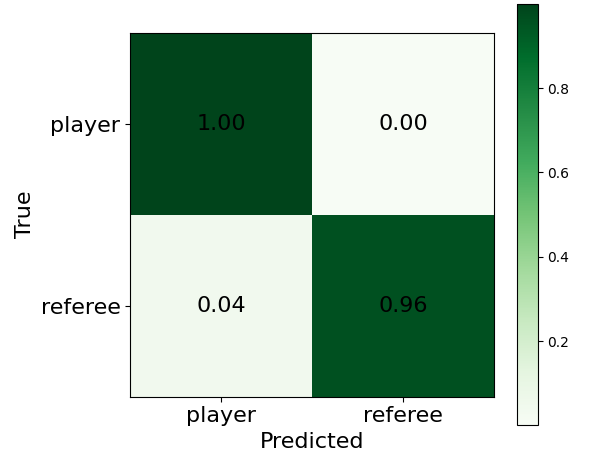
\includegraphics[width=0.8\linewidth]{figures/confusion-player-referee.png}
    \caption{Normalised confusion matrix for the player and referee classes on the test set.}
    \label{fig:cm_player_ref}
\end{figure}

As for the ball, three variants of the detector were compared: the base model trained jointly with players and referee (\textit{baseline}), the model specialised in the ball only (\textit{ball}), and the specialised version with \emph{slicing} inference over patches (\textit{ball\_sliced}). Figure~\ref{fig:pc_ball_models} shows the \emph{Precision--Confidence} curves. Over practically the whole range of thresholds, the specialised models reach a higher precision than the baseline, and the model with \textit{slicing} achieves the best values.

\begin{figure}[H]
    \centering
    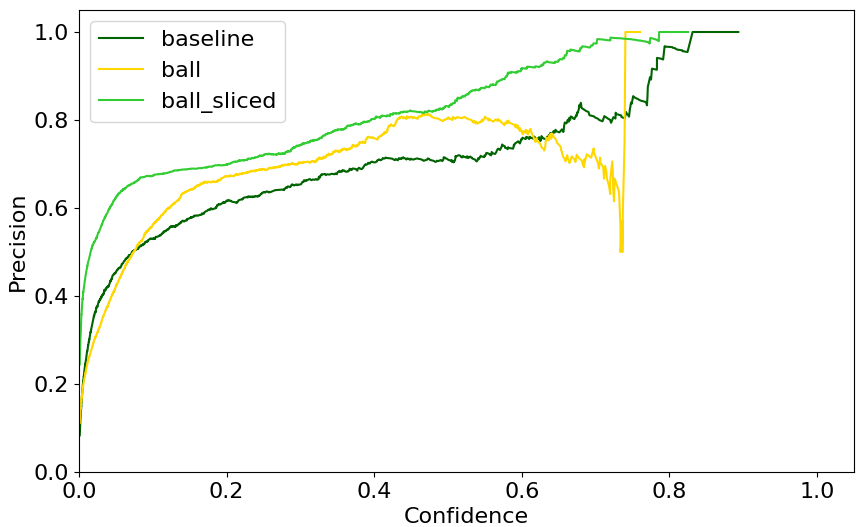
\includegraphics[width=0.95\linewidth]{figures/ball-precision-confidence.png}
    \caption{\emph{Precision--Confidence} curves for the ball detection models: \textit{baseline}, \textit{ball} and \textit{ball\_sliced}.}
    \label{fig:pc_ball_models}
\end{figure}

\subsection{Player grouping and team analysis}

Grouping by appearance was treated as an unsupervised learning problem, so the evaluation was carried out qualitatively. Starting from the visual embeddings obtained with DINOv2 and the per-\emph{track} averaging scheme, the model groups the players into two clusters that consistently correspond to the two teams on the pitch.

In the sequences that were evaluated, the team assignment stayed stable over time, even under partial occlusion or changes in lighting. This makes it possible to colour every \emph{track} with the colour of its team and to keep a clear separation between the two sides of the field.

Figure~\ref{fig:team_assignment} shows an example frame with the final team segmentation, in which the players of each team are labelled correctly.

\begin{figure}[H]
    \centering
    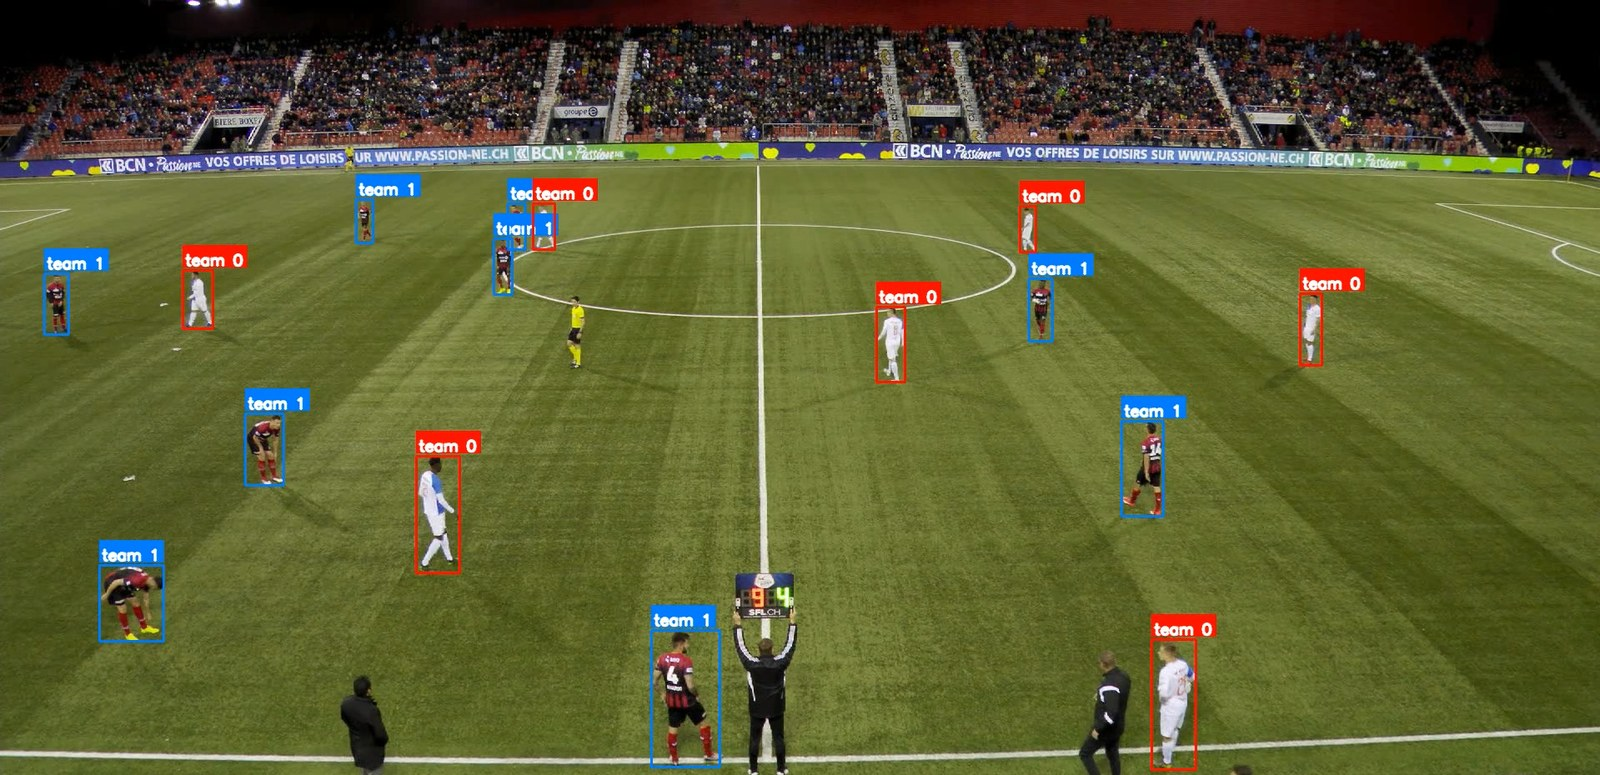
\includegraphics[width=0.9\linewidth]{figures/team-assignment.jpg}
    \caption{Team segmentation example: players coloured according to the assigned \textit{cluster}.}
    \label{fig:team_assignment}
\end{figure}

\subsection{Keypoint detection}
To evaluate keypoint detection accuracy, models trained with \texttt{YOLOv8x} to predict 29 and 57 points respectively were compared on the \textit{test} set provided by SoccerNet. Two groups of metrics were reported in both cases:

\begin{itemize}
    \item \textbf{Average per-point error (RMSE)}: pixel-wise error for every keypoint marked as visible in the \textit{ground truth}.
    \item \textbf{Visibility metrics}: \textit{precision}, \textit{recall}, true positives (TP), false positives (FP) and false negatives (FN), treating any prediction with confidence $>0.4$ as visible.
\end{itemize}

Both models show a consistent pattern in their individual errors. Keypoints placed in structurally well-defined areas, such as the corners of the penalty box and the upper corners of the field, have the lowest RMSE values, around 15--20 px in both models.

The points corresponding to midfield and to the lower touchline, on the other hand, were the most problematic in both architectures. The intersections of the halfway line with the upper and lower edges, as well as the points near the lower touchline, show the largest errors, reaching values close to 300--350 px. This is because these regions are not well-defined corners and are affected by \textit{motion blur} during horizontal camera pans and by partial occlusion. As a consequence, both models are unstable in these areas, which later affects the homography estimation.

\subsubsection*{Comparison between the 29 and 57 keypoint models}

Although the 57-keypoint model produces a more detailed geometric representation, its performance in visibility and consistency was slightly worse than that of the 29-keypoint model.

The visibility metrics for both models are summarised in Table~\ref{tab:visibility_comparison}.

\begin{table}[H]
\centering
\caption{Comparison of visibility metrics between the 29 and 57 keypoint models.}
\label{tab:visibility_comparison}
\vspace{0.2cm}
\begin{tabular}{l c c}
\toprule
\textbf{Metric} & \textbf{29 KP} & \textbf{57 KP} \\
\midrule
Precision & 0.805 & 0.779 \\
Recall & 0.856 & 0.803 \\
TP & 13821 & 34150 \\
FP & 3347 & 9697 \\
FN & 2317 & 8369 \\
\bottomrule
\end{tabular}
\end{table}

Note that the absolute TP, FP and FN values are not directly comparable across architectures, since the 57-keypoint model evaluates a larger number of points per image. For that reason, the comparison between models is based mainly on normalised metrics such as precision and recall.

Overall, the 57-keypoint model produced a larger proportion of low-confidence points, which hurts frame-to-frame stability. The 29-keypoint model, although geometrically less expressive, gave more robust and stable predictions.

The final pipeline therefore uses the 29-keypoint model.

\vspace{2mm}

Despite the good results on the test set, a significant difference in performance was observed when the model was applied to continuous video sequences coming from a different domain: matches from other leagues, different lighting conditions and camera angles that were not seen during training. Good results on still images notwithstanding, inference on video was highly unstable over time.

This can be seen in Figure~\ref{fig:still_vs_video}. The poor performance is attributed to how different the images are compared to the training set, to the image quality degradation inherent to video, and to the \textit{blur} introduced by camera pans.

\begin{figure}[H]
    \centering

    \begin{subfigure}{\linewidth}
        \centering
        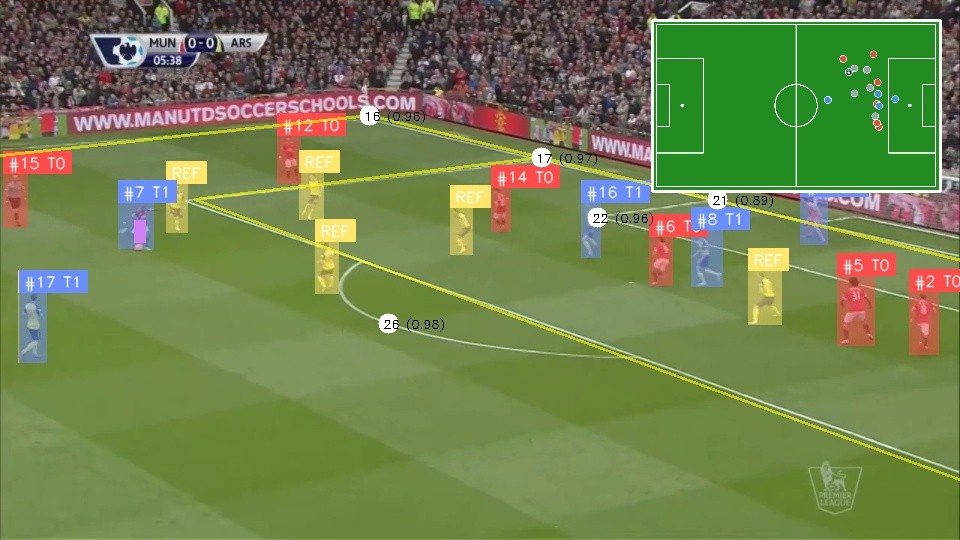
\includegraphics[width=\linewidth]{figures/homography-still.jpg}
        \caption{Result on the test set (still image).}
        \label{fig:result_still}
    \end{subfigure}

    \par\bigskip

    \begin{subfigure}{\linewidth}
        \centering
        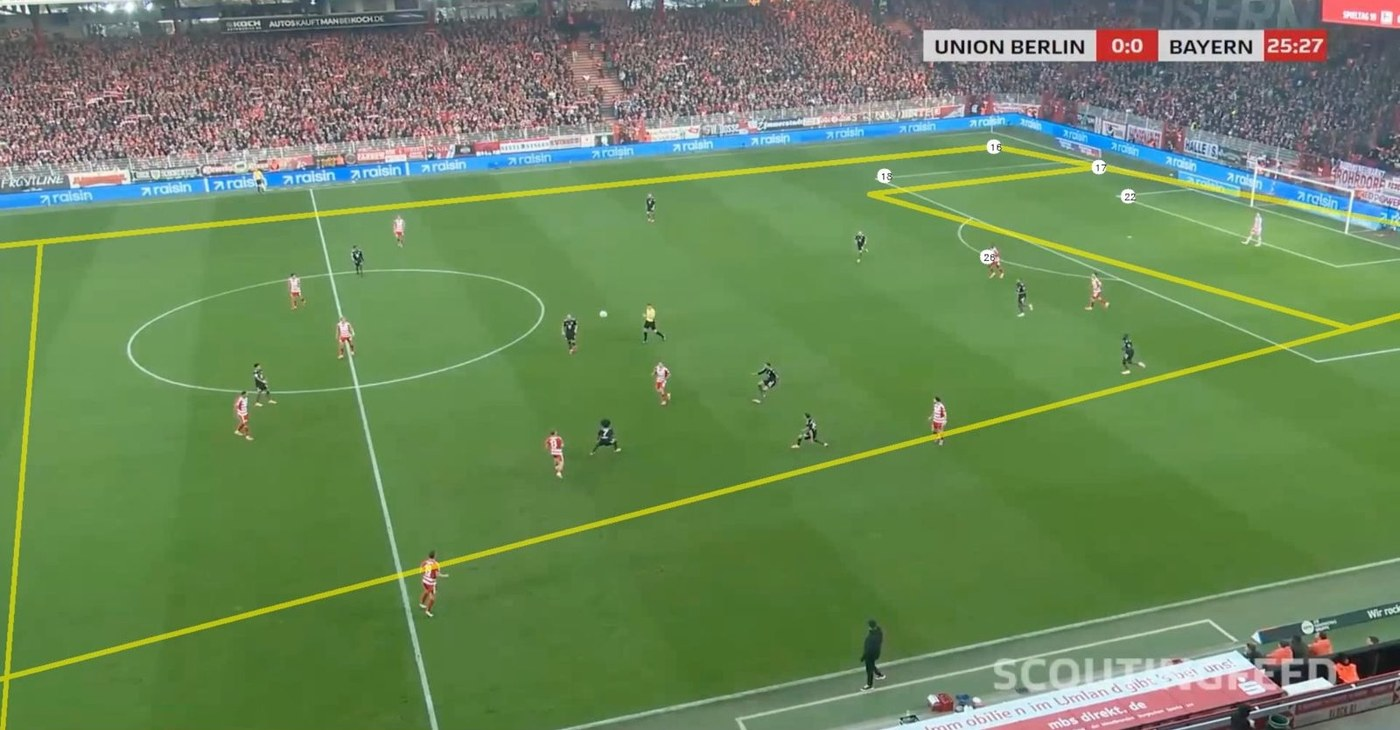
\includegraphics[width=\linewidth]{figures/homography-video.jpg}
        \caption{Result on video.}
        \label{fig:result_video}
    \end{subfigure}

    \caption{Performance comparison. (a) shows the accuracy under ideal conditions. (b) shows the instability and the loss of points caused by motion blur and low image quality.}
    \label{fig:still_vs_video}
\end{figure}

\subsection{Homography estimation and projection}

Homography estimation was directly tied to the performance of keypoint detection. The drop in keypoint detection accuracy on video had an immediate impact on the homography computation. Since the projection matrix is highly sensitive to the destination coordinates, it turned out to be very inconsistent over time. Visually this showed up as reprojection errors on the radar, where player positions jumped or fell out of alignment with the lines of the virtual pitch.

Even so, although the projection was noisy (especially during pans), the system recovered almost immediately once the camera held still or moved smoothly. Under those conditions the model was able to recover high-confidence detections, so the homography converged correctly and the jitter in the tactical view disappeared.

\subsection{Discussion and interpretation}

The \textit{pipeline} developed here demonstrates that detection, tracking and appearance analysis modules can be integrated to produce a metric representation of the game. Performance was asymmetric across the stages: object detection and team classification proved highly consistent and robust to occlusion, whereas the geometric reconstruction turned out to be critically sensitive to the quality of keypoint detection.

The results validate the effectiveness of the proposed approach, but they show that estimating the homography on video calls for additional considerations. Factors such as the symmetry of the pitch introduce positional ambiguities, and the frequent lack of visible points in tight shots makes it impossible to have the redundancy needed to filter out detection errors. This indicates that the stability of the metric system depends on several factors, not only on the spatial accuracy of the detector.

\end{multicols}
